\chapter{Results and Discussion}\label{chap:results}
\begin{overview}
  The results of this project is summarized and discussed in this chapter.
  Implementation of the method to the case studies and test problems are presented.
  General results concerning the constraint set fitting are also discussed.
  A final section is devoted to discussing the rationale behind future expansions of constraint set fitting.
\end{overview}

\section{Case studies}
The method of systematic constraint handling (as outlined in chapter~\ref{chap:conhand}) is applied to the case studies.
For ease of graphical representation, only $2\times2$ systems are evaluated.
It should however be noted that the proposed method applies to higher order systems -- with the current exception of arbitrary constraint set fitting as discussed in section~\ref{sec:fittingaccuracy}.
\subsection{Level and flow rig}
\subsubsection{Input/Output spaces}
The input and output spaces for the level and flow rig are shown in figure~\ref{fig:flowaisaos}.
From the intersection of the AOS and the DOS, the OI is calculated as 0.338.

\begin{figure}[htbp]
  \centering
    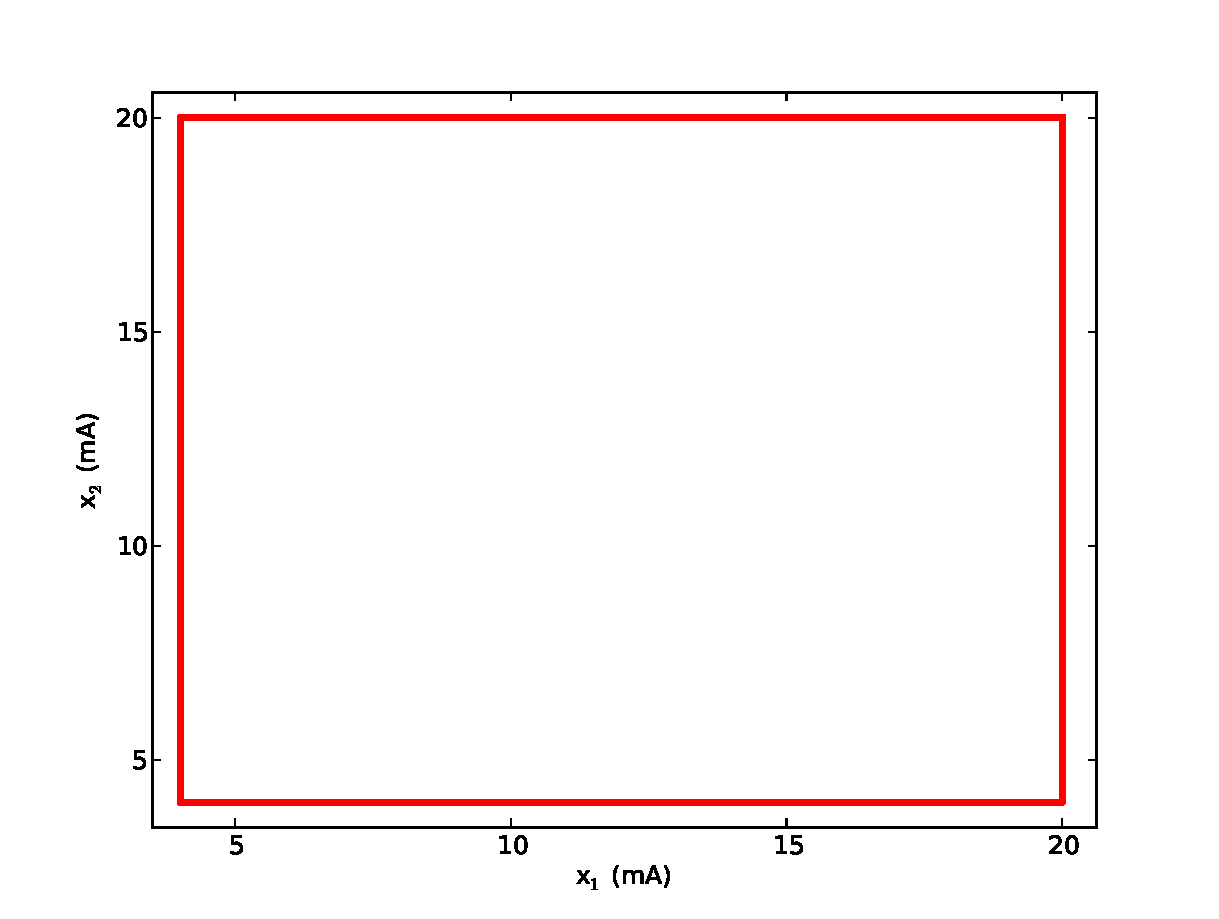
\includegraphics[width=7.8cm]{graph/flowais.pdf}
    %\qquad
    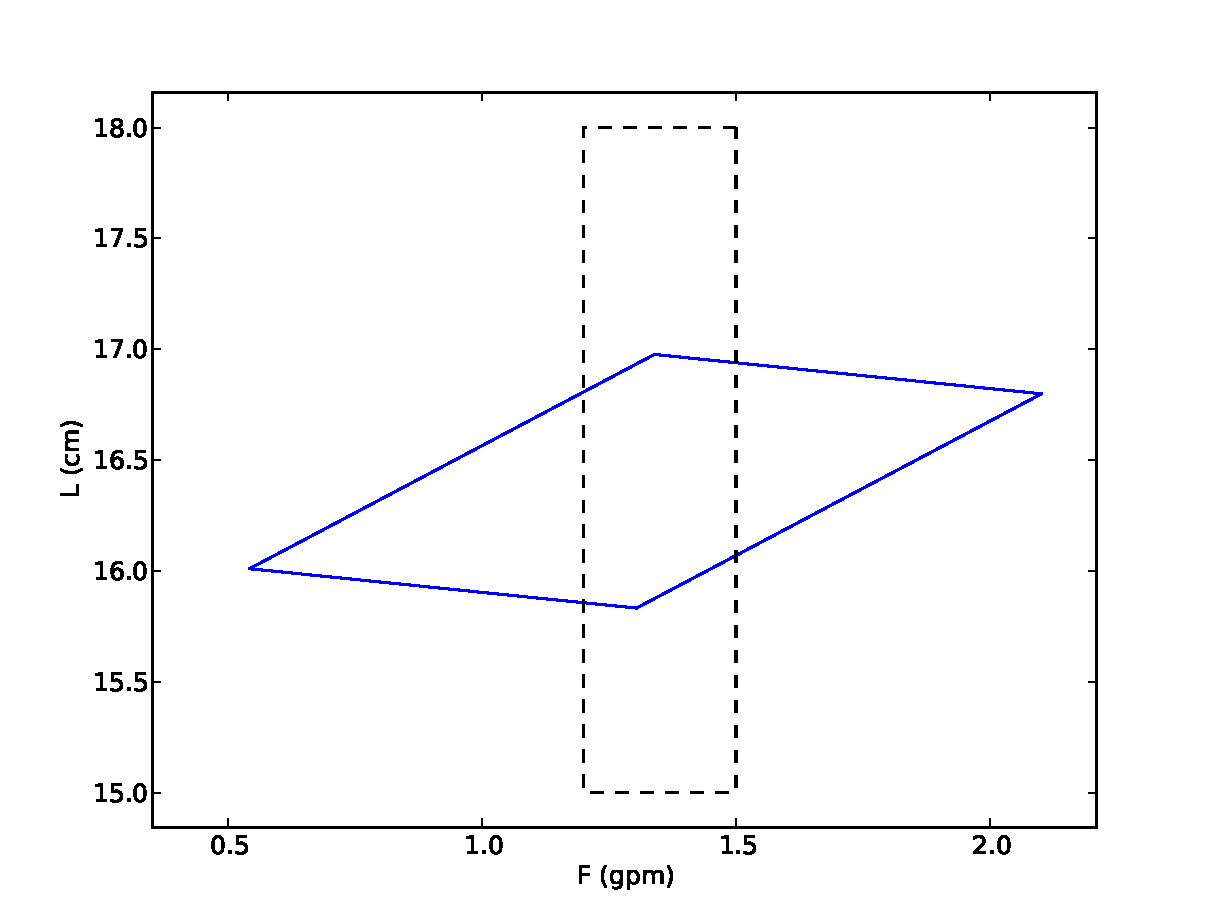
\includegraphics[width=7.8cm]{graph/flowaos.pdf}
  \caption[AIS, AOS and DOS of the level and flow rig]{AIS (left), AOS and DOS (right) for the level and flow rig.}
  \label{fig:flowaisaos}
\end{figure}

\subsubsection{Set fitting}
It is clear that the level range expectations of this process is too ambitious.
Decreasing these limits will not affect the control adversely, as the model suggests that these upper and lower level limits are not attainable.
Figure~\ref{fig:flowfitbox} shows the fitting of upper/lower constraints within the intersection of the AOS and the DOS.
The dark box represents the largest operating region (described only by high/low limits on the outputs) which are within the original DOS and the AOS.
This procedure increases the OI to 1 and presents tighter bounds that are all feasible.

\begin{figure}[htbp]
  \centering
    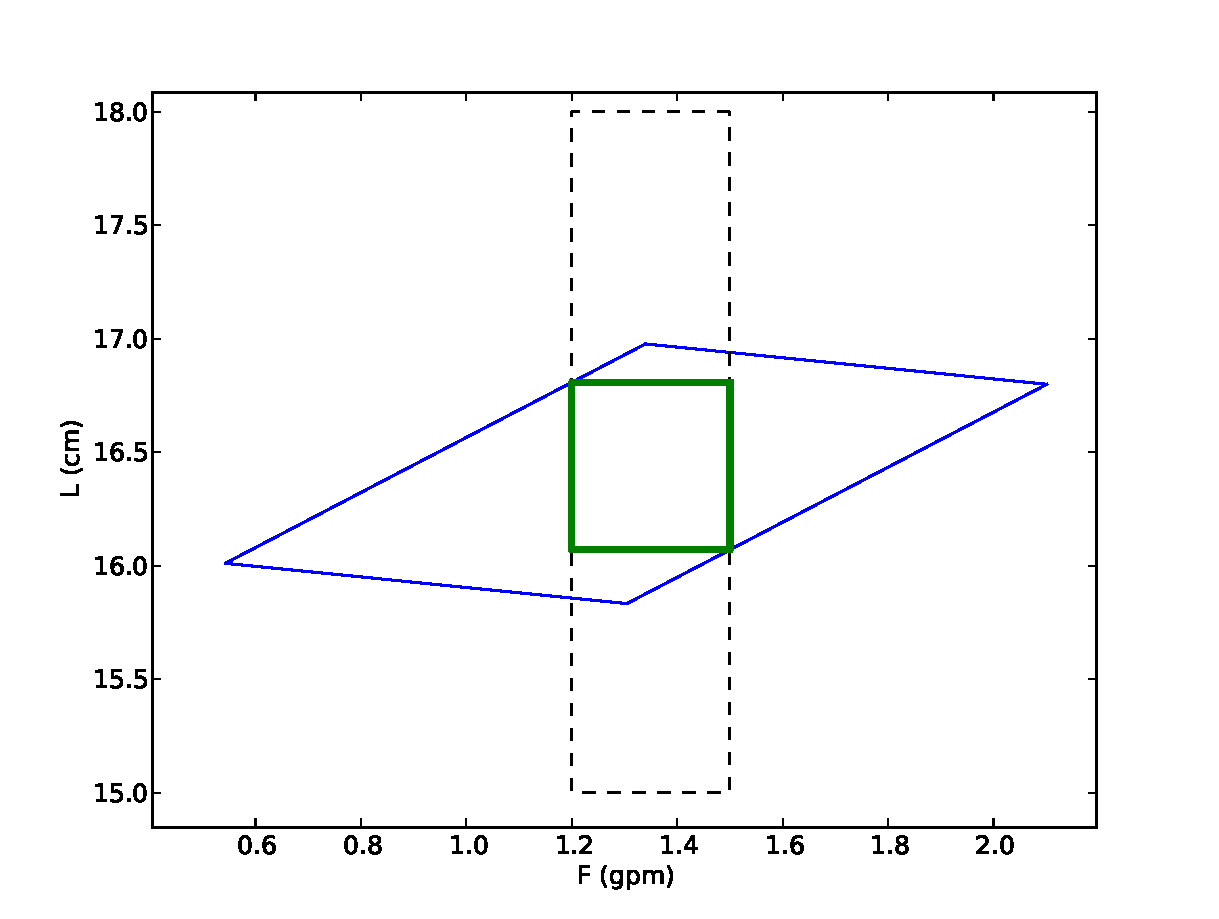
\includegraphics[width=\fullwidth]{graph/flowfitbox.pdf}
  \caption{Fitted high/low constraints in the AOS/DOS intersection.}
  \label{fig:flowfitbox}
\end{figure}

\subsubsection{Constraint changes}
It is typical of operators to change constraints during the operation of processes.
Usually, constraints are tightened on outputs/inputs.
It is intuitive that constraint tightening in the output space has a corresponding tightening effect in the input space, but the extent thereof isn't immediately clear.
The same reasoning applies to the changing of input constraints.

As an example, the newly fitted upper and lower bounds of figure~\ref{fig:flowfitbox} is considered and the effect of this constraint change in the input space investigated.
Figure~\ref{fig:flowconsinput} shows the original AIS and DIS, along with the new DIS (the dark dashed box) that corresponds to the changed constraints.
This figure also serves to confirm that the newly fitted constraints on the outputs correspond to a fully attainable region in the input space.

\begin{figure}[htbp]
  \centering
    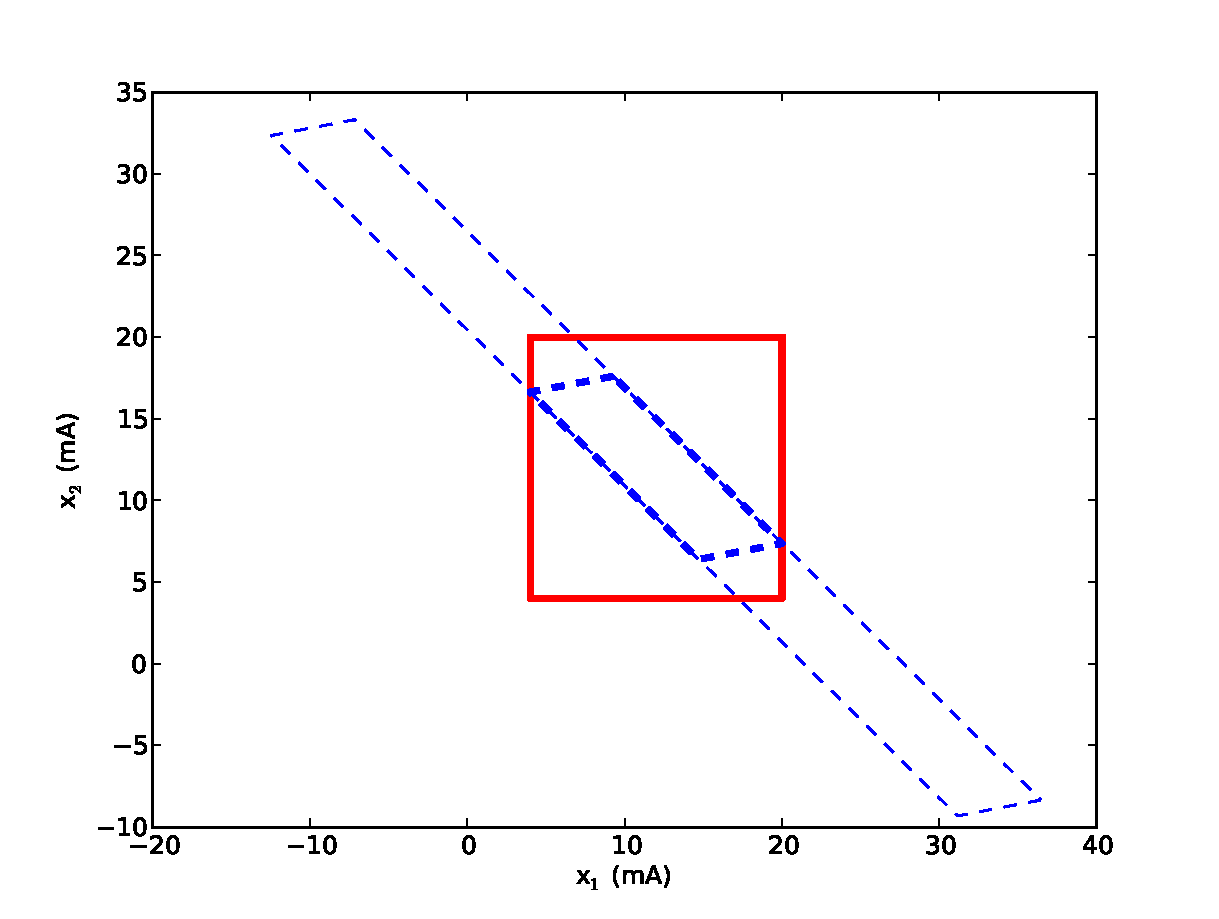
\includegraphics[width=\fullwidth]{graph/flowconsinput.pdf}
  \caption[AIS, DIS and newly fitted DIS of level and flow rig]{Newly fitted constraint set shows feasible input constraints as opposed to those of the original DOS.}
  \label{fig:flowconsinput}
\end{figure}

The unattainable limits of the DOS are just as clear in the input space (DIS).
To quantify the tightening of the inputs, the OI of \citet{vinsonphd} can be used, although, this has the obvious downside of increasing as the DIS moves to the inside of the AIS, regardless of the DIS's actual size.
Another possibility is a ratio of hypervolumes for the original attainable part of the DIS and the attainable part of the new DIS ($DISn$).
In figure~\ref{fig:flowconsinput} this corresponds to
\begin{equation}
  \label{eq:inputclamp}
  1-\frac{\mu(AIS \cap DISn)}{\mu(AIS \cap DIS)} = 0.27 \notag
\end{equation}
where $\mu$ is a function to calculate the hypervolume of a space.
This indicates that the attainable movement on the inputs has effectively been tightened by 27\%. 

\subsubsection{Constraint types}
As mentioned in section~\ref{sec:commercialmpc}, the only constraint validation done by both RMPCT and DMCPlus is checking whether the operator constraints are within the engineering constraints.

The engineering constraints are typically set by the physical constraints of the system.
Figure~\ref{fig:flowcontypes} shows the AOS (as determined by the AIS) and original DOS, along with the physical constraints of the system (table~\ref{tab:flowopcon}).
It is clear that with only checking against physical constraints, specification of a DOS that is completely unattainable is possible.

Figure~\ref{fig:flowcontypes} also shows the fitting of a revised set of engineering limits with a safety factor of 20\%.

\begin{figure}[htbp]
  \centering
    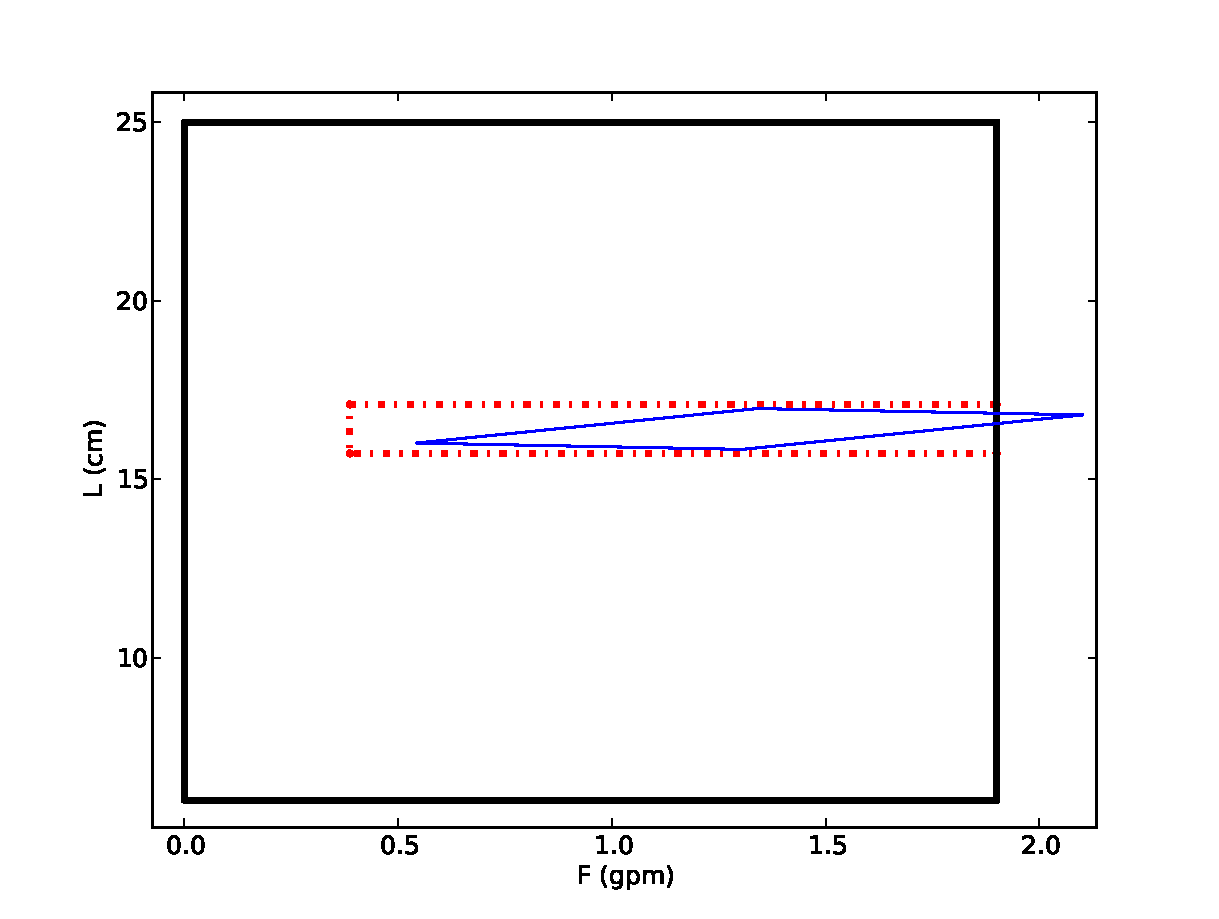
\includegraphics[width=\fullwidth]{graph/flowcontypes.pdf}
  \caption[Physical constraint region of level and flow rig]{Physical constraint region, AOS and revised engineering limits (with a 20\% safety factor) of the level and flow rig.}
  \label{fig:flowcontypes}
\end{figure}

\subsubsection{MPC interfacing}
Table~\ref{tab:flowsummary} summarises the results obtained for the level and flow rig.
This table serves to illustrate the application of the when using a commercial MPC package.
The operator interfaces for RMPCT and DMCPlus, shown in figures~\ref{fig:ssrmpctoperator} and \ref{fig:ssdmcplusoperator} respectively, will be used to enter these constraints.
For RMPCT (figure~\ref{fig:ssrmpctoperator}) the shaded columns labeled 'Low Limit' and 'High Limit' are used.
For DMCPlus (figure~\ref{fig:ssdmcplusoperator}) the column labeled 'Lower Limit' and 'Upper Limit' are used.

\begin{table}[htbp]
  \centering
  \begin{tabular}{llll}
    \toprule
    \multicolumn{2}{c}{Variable} & \multicolumn{2}{c}{Fitted constraints}\\
    && Low & High\\ 
    \midrule
    Outputs &$F~(\text{gpm})$ & 1.2 & 1.5 \\
            &$L~(\text{cm})$  & 16.1 & 16.8 \\
    \bottomrule
  \end{tabular}
  \caption{Summary of results obtained for level and flow rig.}
  \label{tab:flowsummary}
\end{table}


\subsection{Laboratory distillation column}
\subsubsection{Input/Output spaces}
From the data in table~\ref{tab:columnopcon} and equation~\ref{eq:columnmodel} the AIS and AOS of the laboratory distillation column can be generated as shown in figure~\ref{fig:columnaisaos}.
Take note that the operating limits for $R$ is used to construct the AIS as values outside of this range (although) possible cause the validity of the model to diminish.
The DOS, as described by the operating range in table~\ref{tab:columnopcon}, is also shown.

\begin{figure}[htbp]
  \centering
    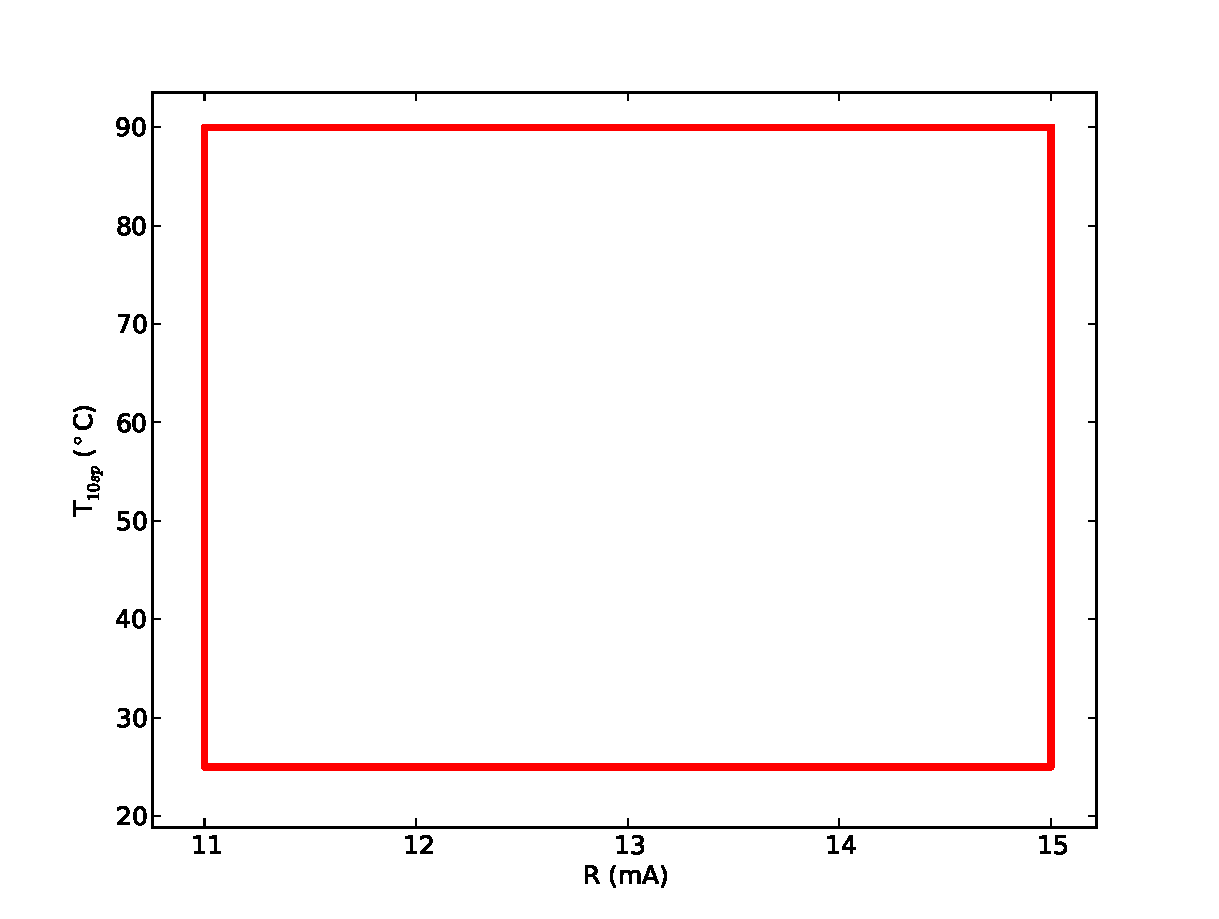
\includegraphics[width=7.8cm]{graph/columnais.pdf}
    %\qquad
    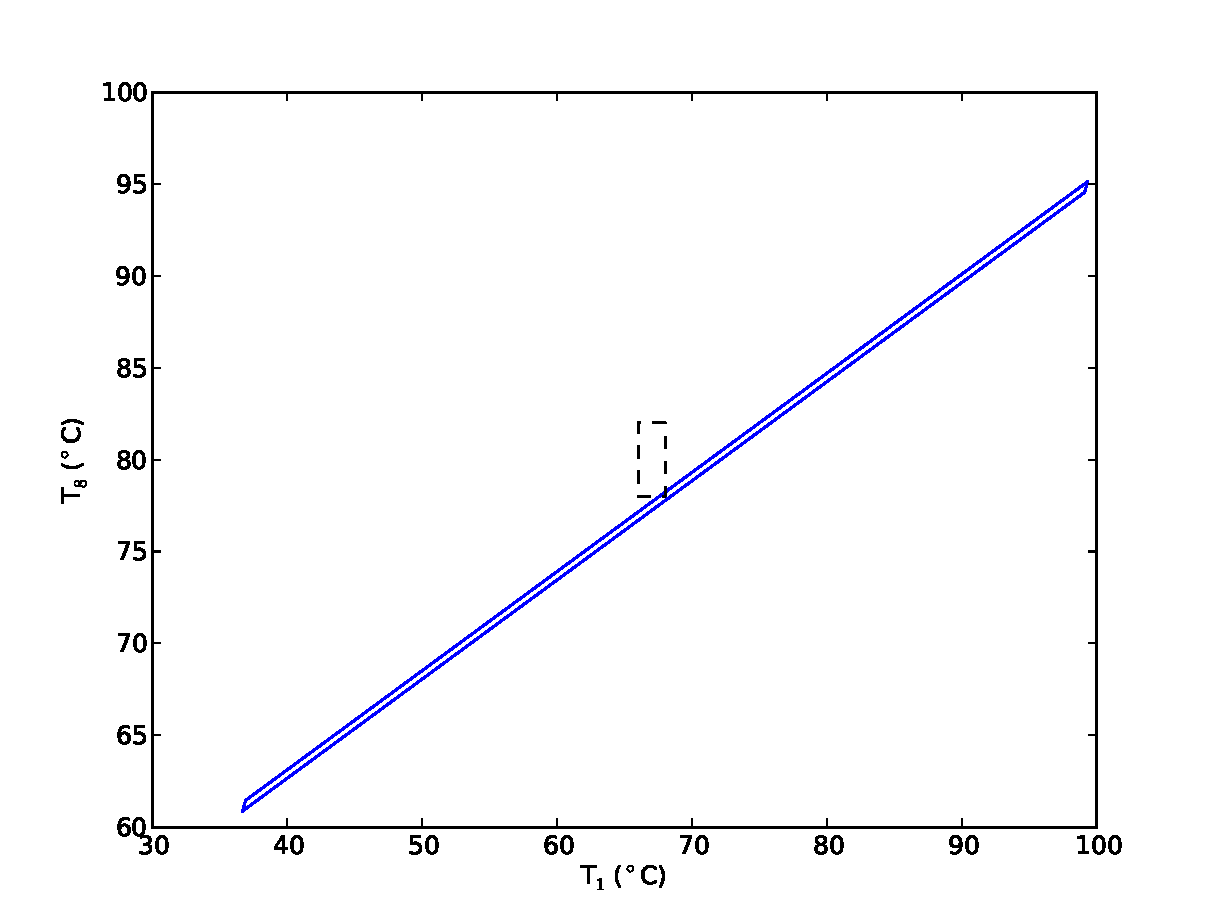
\includegraphics[width=7.8cm]{graph/columnaos.pdf}
  \caption[AIS, AOS and DOS of the laboratory distillation column]{AIS (left), AOS and DOS (right) of the laboratory distillation column.}
  \label{fig:columnaisaos}
\end{figure}

Figure~\ref{fig:columnaosfocus} focuses on the intersection of the AOS and the DOS.
The calculated OI is 0.006 which confirms that only a very small operating region within the DOS is attainable.
It is also clear that the upper limit of 82$\degrees{C}$ on $T_8$ is unrealistic as the maximum value of $T_8$ (in the operating region) is only 78.2$\degrees{C}$.

\begin{figure}[htbp]
  \centering
    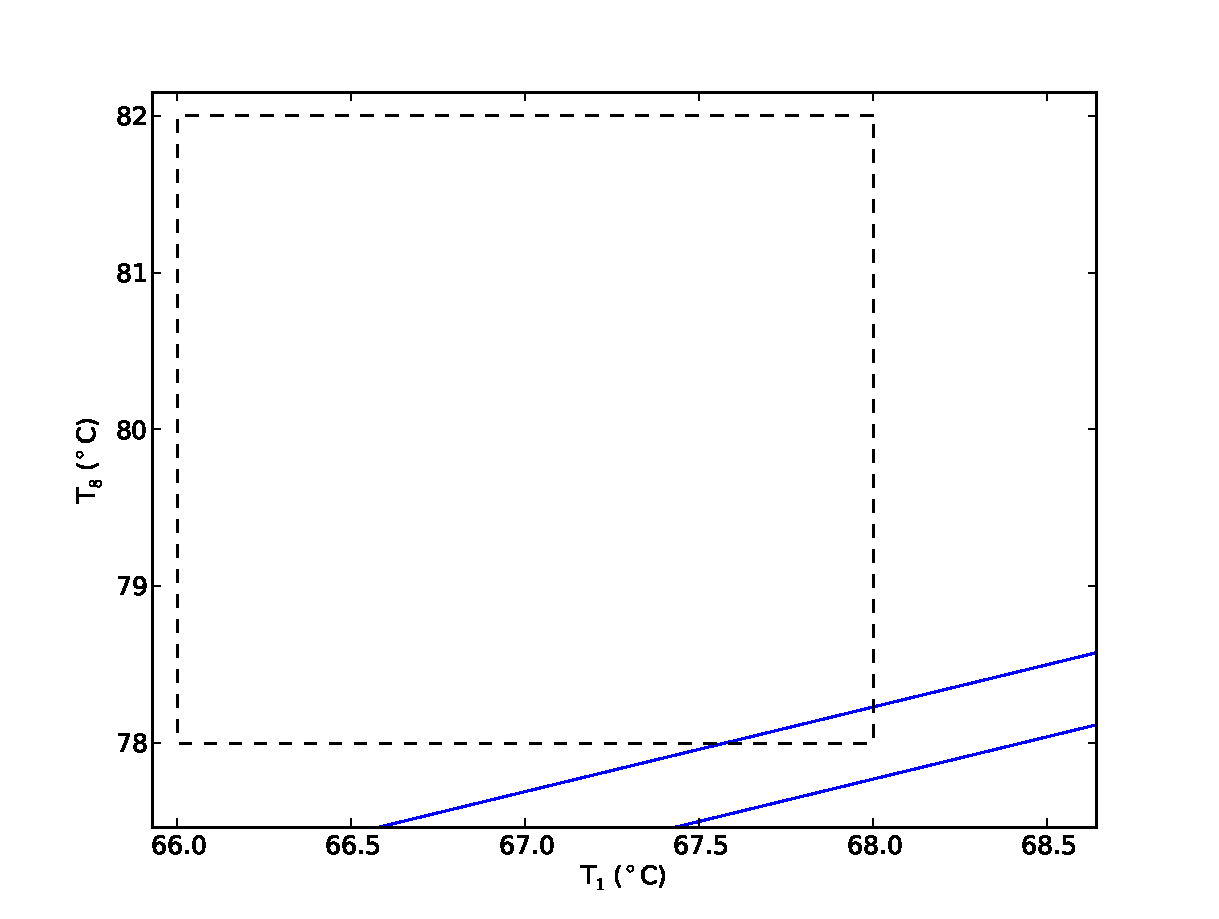
\includegraphics[width=\fullwidth]{graph/columnaosfocus.pdf}
  \caption[AOS and DOS intersection of the laboratory distillation column]{The AOS and DOS intersection shows a very small operating region.}
  \label{fig:columnaosfocus}
\end{figure}

\subsubsection{Set fitting}
Figure~\ref{fig:columnfitbox} focuses even closer on the AOS/DOS intersection.
The constraints representing the intersection (dark triangle) and a fitted set of high/low limits (dark dashed box) is also shown.
The fitted limits within the intersection shows that the operating region is essentially an operating point with temperatures only having a span of about 0.1$\degrees{C}$.
In practice the DOS would be adjusted, but for the sake of illustrating the outputs of the method, the DOS will be kept as is.
  
\begin{figure}[htbp]
  \centering
    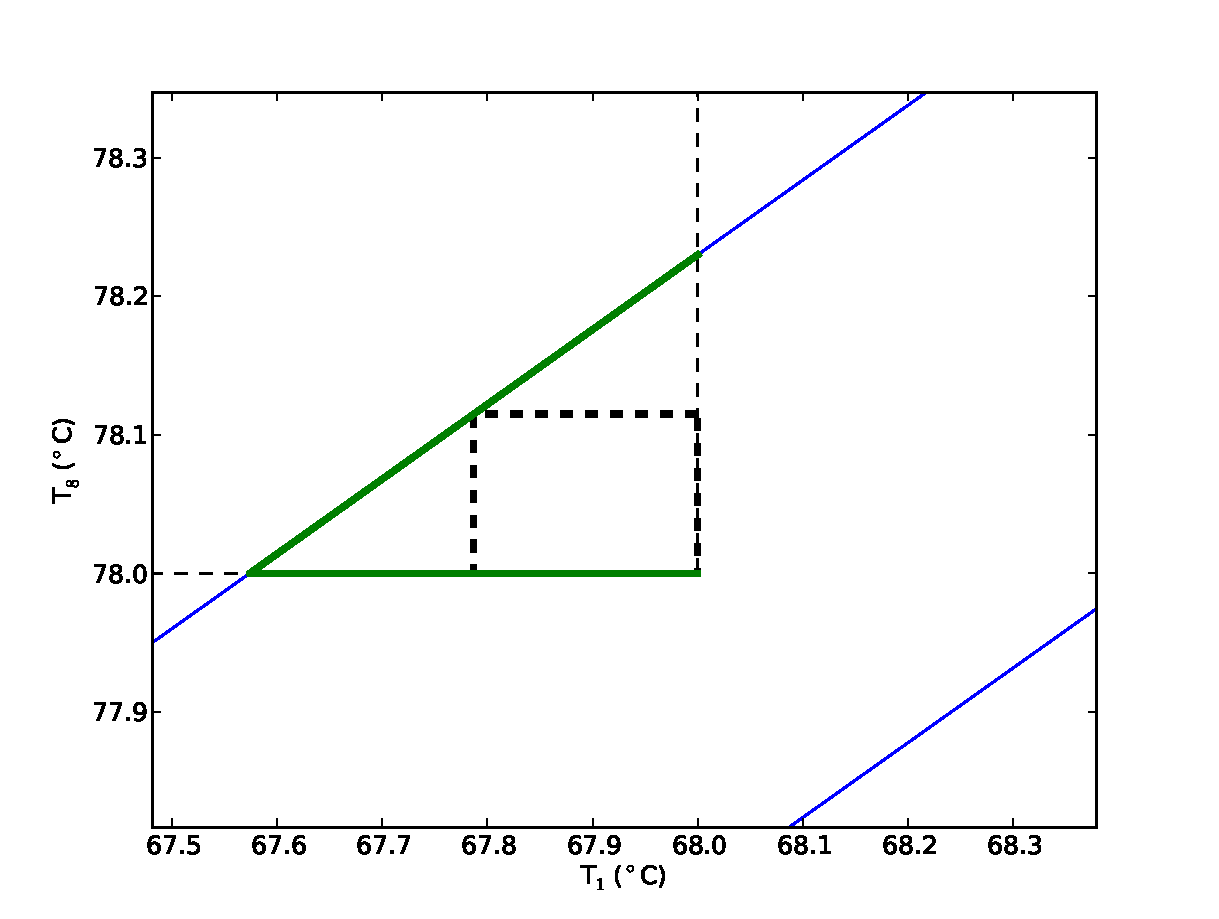
\includegraphics[width=\fullwidth]{graph/columnfitbox.pdf}
  \caption[Fitted constraints for the laboratory distillation column]{Intersection of AOS and DOS with fitted high/low limits for the column tray temperatures.}
  \label{fig:columnfitbox}
\end{figure}

\subsubsection{Constraint reformatting}
Rather than using the high/low limits as shown in figure~\ref{fig:columnfitbox}, the constraints describing the whole intersection will be used.
This set of constraints need to be reformatted to be compatible with commercial MPC packages, as they only accept high/low limits.

A pseudo-variable needs to be added to the process model and the diagonal constraint ($0.88T_8-0.47T_1\leq 36.56\degrees{C} $) needs to be expressed as a high/low limit on this pseudo-variable.

Naming the new output $y_1$ and augmenting the process model matrix as shown in equation~\ref{eq:columnnewmodel} allows for the diagonal (linear) constraint to be expressed simply as {$y_1~\leq~36.56\degrees{C}$}.

\begin{equation}
  \label{eq:columnnewmodel}
  G_{col-new}= \bpm -0.0575 & 0.96 \\       % T1
                  -0.146  & 0.518 \\      % T8
                   0.0956 & 1.30 \\ \epm  %y1
\end{equation}

\subsubsection{MPC interfacing}
As with the level and flow rig, the operator interfaces (figures~\ref{fig:ssrmpctoperator} and \ref{fig:ssdmcplusoperator}) are used to set the constraints for the system.
The modelling interfaces (figures~\ref{fig:ssrmpctmodel} and \ref{fig:ssdmcplusmodel}) are used to augment the model for the addition of unmeasured variables.

\section{Constraint set fitting}
The fitting of constraint sets, which form a large part of this dissertation, is discussed separately.
Observations made whilst studying the fitting of constraint sets, which could lead to future research is discussed in section~\ref{sec:setfitfuture}.

\subsection{Solution times}
The use of constrained, gradient-based solvers proved to be significantly faster than unconstrained solvers.
Inconsistent gradient information does, however, hamper their use.

Figure~\ref{fig:cubefittime} compares the solution times of SLSQP and simplex for rectangular set fitting.
Arbitrary sets with three constraints on two variables were generated and a high/low constraint set on the two variables were fitted.

\begin{figure}[htbp]
  \centering
    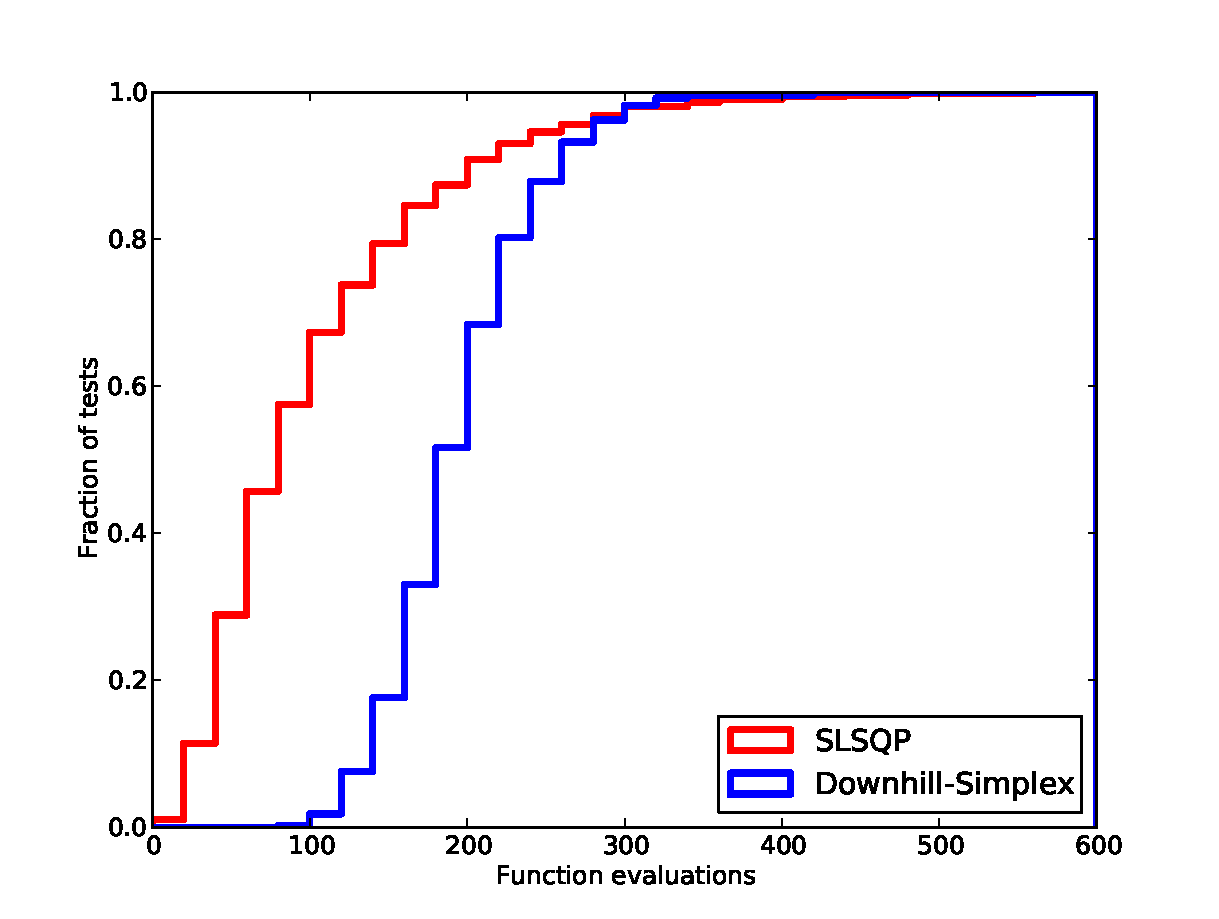
\includegraphics[width=\fullwidth]{graph/cubefittime}
  \caption[SLSQP and simplex calculation time comparison]{Cumulative plot of function evaluations showing faster execution of SLSQP vs simplex}
  \label{fig:cubefittime}
\end{figure}

Fitting a constraint set of an arbitrary size was unsuccessful using constrained, gradient-based solvers.
Possible reasons for this is inconsistent gradient information regarding the position of vertices outside the initial set and the superfluous degrees of freedom present in the problem formulation.

\subsection{Accuracy}\label{sec:fittingaccuracy}
The solutions for high/low constraint set fitting resulted in an optimal answer for each test.
The fitting of arbitrary sized constraint sets suffered from accuracy issues due to the high dependence on the starting point.
As mentioned in the preceding section, due to problems with the unconstrained, gradient-based solvers, only simplex was used for the fitting of arbitrary sets.

\subsubsection{Two variable systems}\label{sec:2dfitting}
For these tests, a 3-constraint set was fitted into a 4-constraint set.
The initial set was chosen to be rectangular (high/low limits) to enable the algebraic calculation of the optimal fitted set.
The optimal solution is 50\% of the volume (area in 2 dimensions) of the initial constraint set.
Figure~\ref{fig:arbfitaccuracy2d} shows the accuracy of this fitting test.
It can be seen that 80\% of the solutions were within 10\% of the optimal solution.
\begin{figure}[htbp]
  \centering
    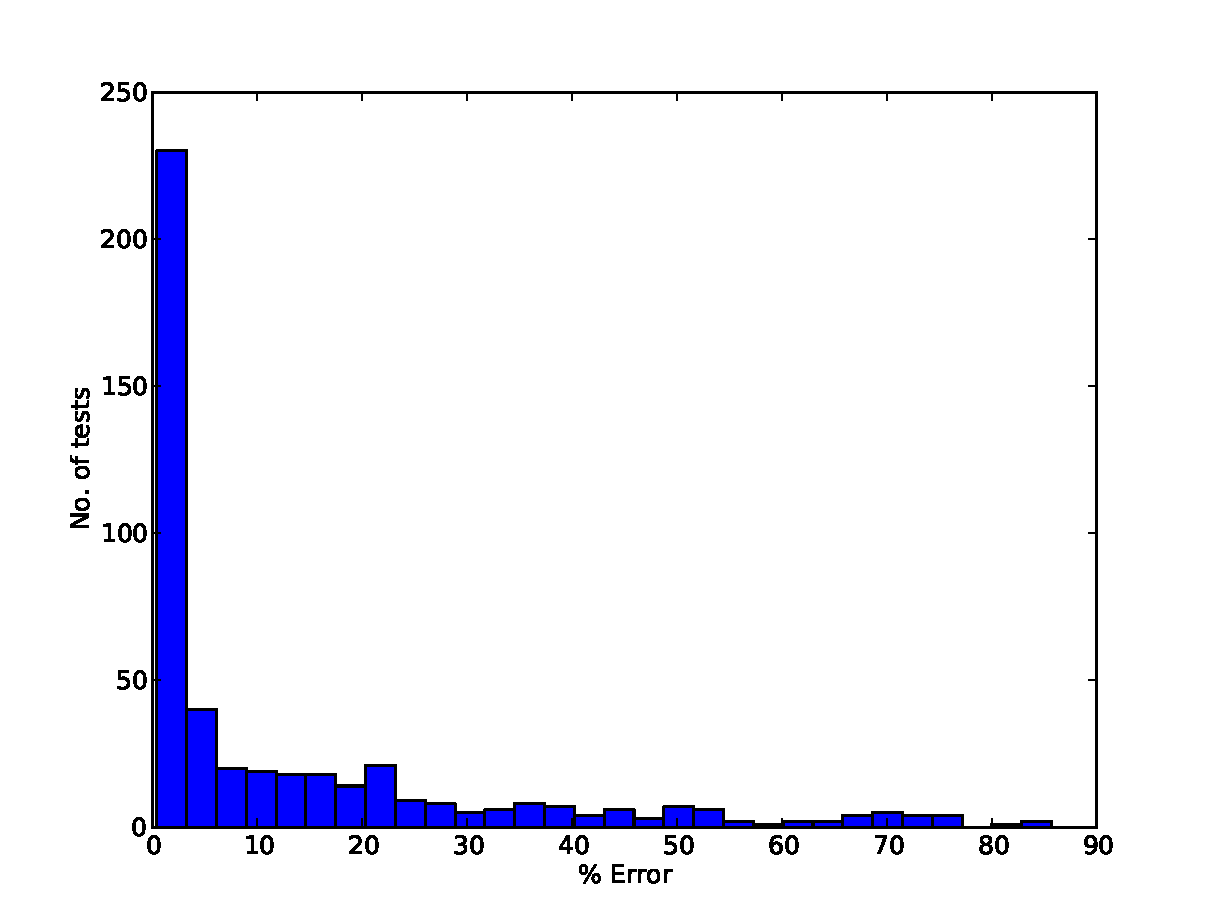
\includegraphics[width=\fullwidth]{graph/arbfitaccuracy2d.pdf}
  \caption[Accuracy of constraint set fitting for 2 variables]{Accuracy of fitting results for a 3-constraint set into a 4-constraint set.}
  \label{fig:arbfitaccuracy2d}
\end{figure}

To increase the accuracy, a multi-start approach was taken where 25 random starting points are generated.
The largest volume set (of the 25 generated) was then used for the fitting.
Figure~\ref{fig:arbfitaccuracy2dmulti} shows the improvement in accuracy with this method.

\begin{figure}[htbp]
  \centering
    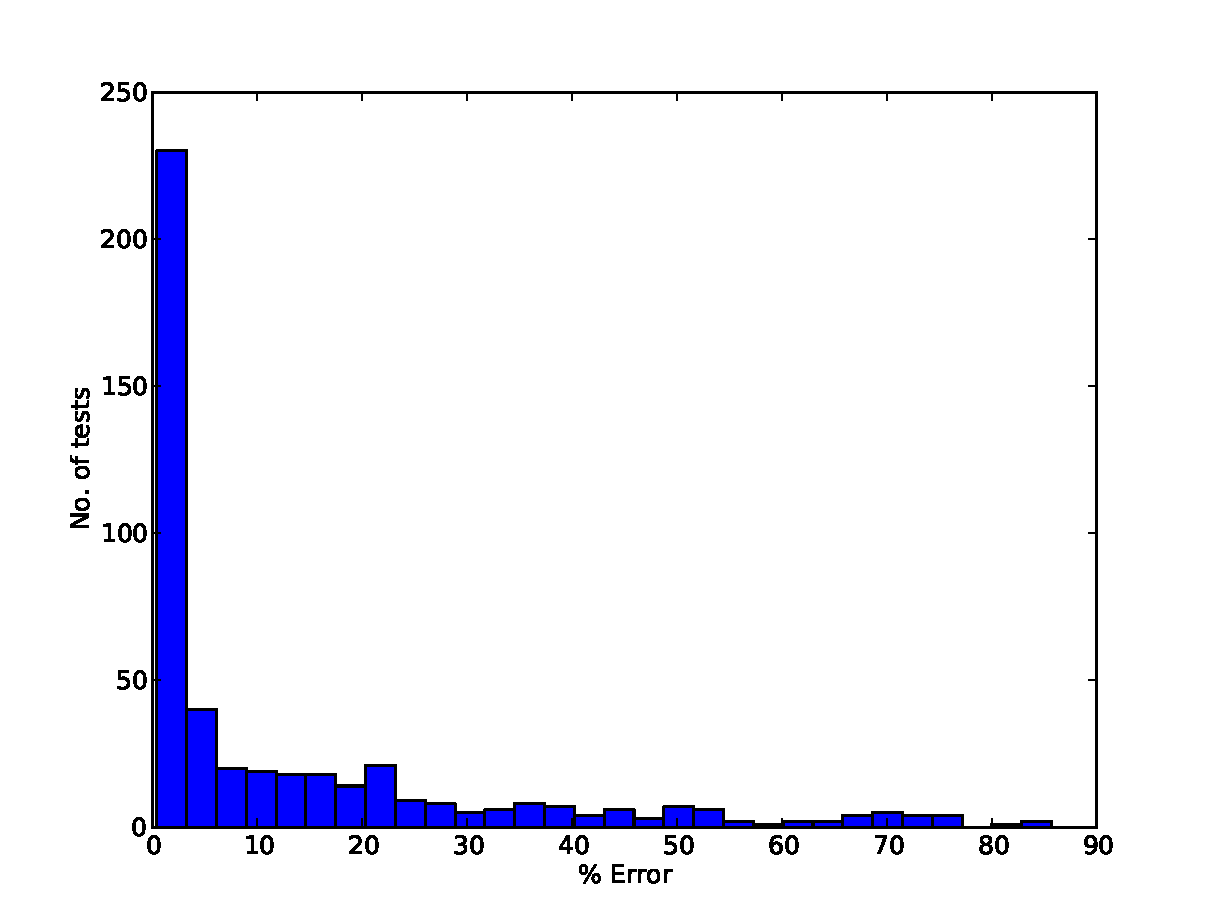
\includegraphics[width=\fullwidth]{graph/arbfitaccuracy2d.pdf}
  \caption[Accuracy of constraint set fitting for 2 variables (multi-start)]{Accuracy increase from the fitting results in figure~\ref{fig:arbfitaccuracy2d} when using a multi-start approach.}
  \label{fig:arbfitaccuracy2dmulti}
\end{figure}
% REPLACE WITH REAL FIGURE

\subsubsection{Three variable systems}
For the three variable tests, a 4-constraint set was fitted into a 6-constraint set.
The initial constraint set was chosen to be a 3-dimensional cube -- again to allow for calculation of the optimal solution.
This test (in geometric terms) results in fitting a tetrahedron into a cube; the optimal solution is 33.33\% of the volume of the cube.
Figure~\ref{fig:arbfitaccuracy3d} shows the accuracy of this test.

\begin{figure}[htbp]
  \centering
    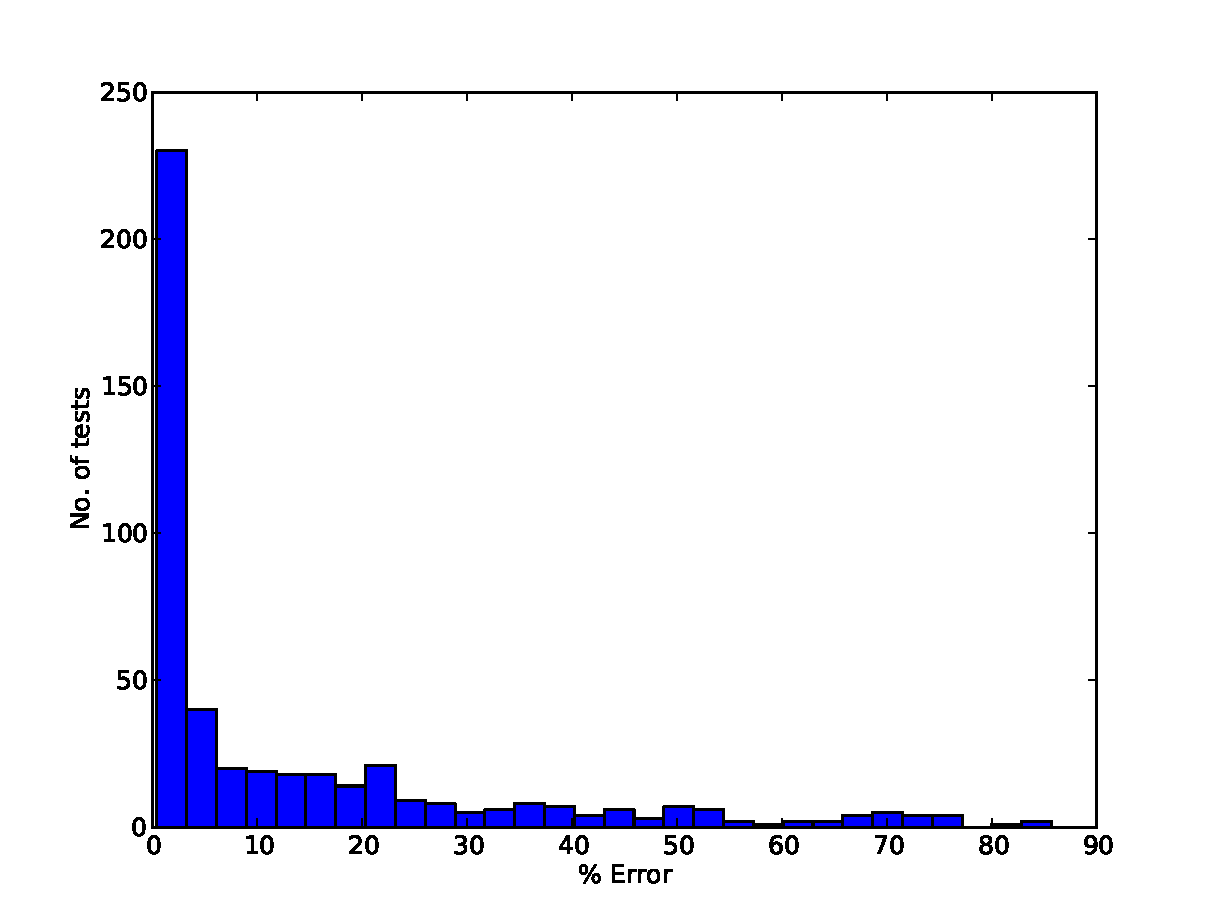
\includegraphics[width=\fullwidth]{graph/arbfitaccuracy2d.pdf}  
  \caption[Accuracy of constraint set fitting for 3 variables]{Low accuracy is obtained for higher dimensional fitting of constraint sets.}
  \label{fig:arbfitaccuracy3d}
\end{figure}

The low accuracy (even when using a multi-start approach) can be ascribed to the increased degrees of freedom and the ill conditioning of the problem.

\subsection{Set fitting expansion}\label{sec:setfitfuture}
The graphs shown in figure~\ref{fig:equaloifits} show a few optimal solutions obtained from the tests of section~\ref{sec:2dfitting}.
It can be noted that even though the sets are not equal, the output operability index \citep{vinsonphd} calculated for all of them are equal.
\begin{figure}[htbp]
  \centering
    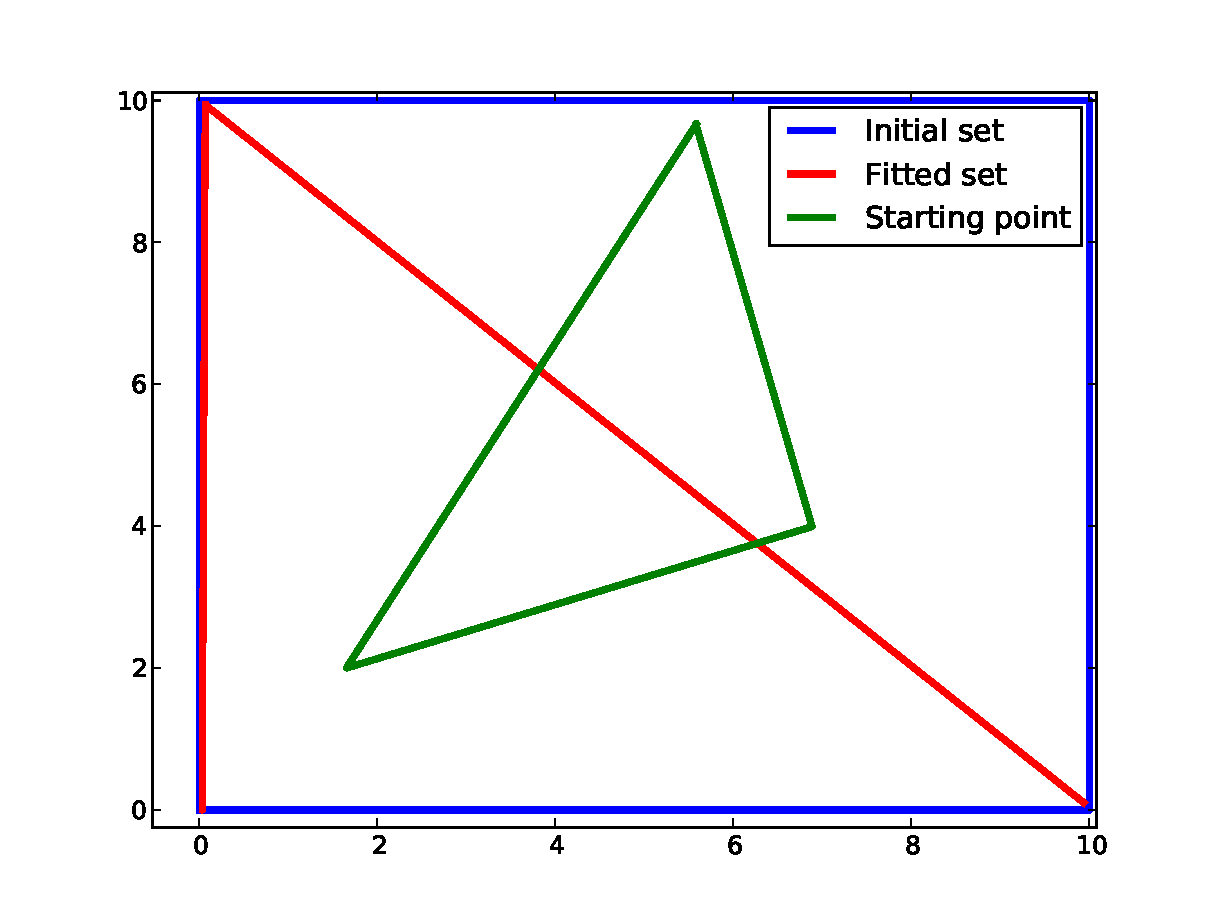
\includegraphics[width=7.8cm]{graph/2dfit1.pdf}
    %\qquad
    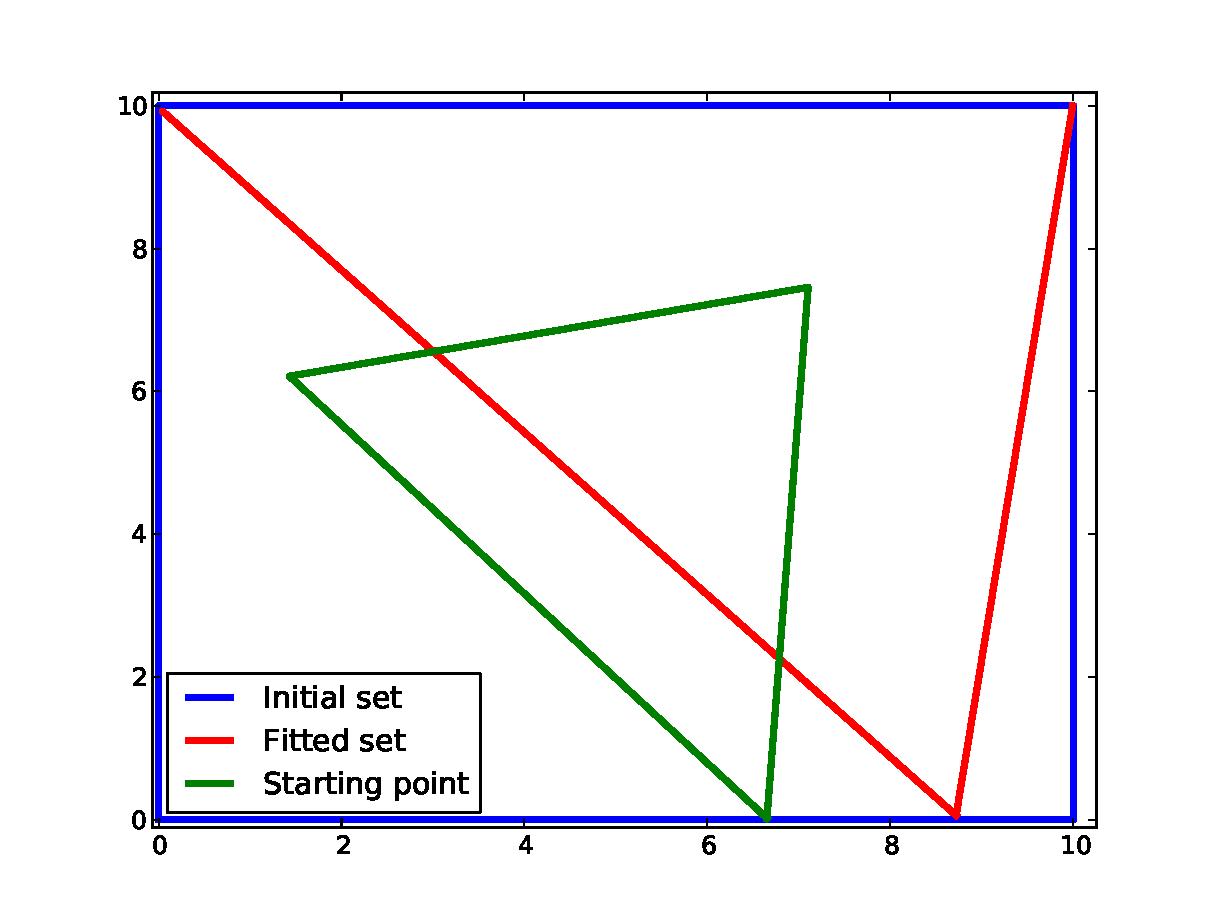
\includegraphics[width=7.8cm]{graph/2dfit2.pdf}
  \caption[Equal size constraint set fits]{Different sets fitted with an equal size and equal calculated Operability Index.}
  \label{fig:equaloifits}
\end{figure}

From these results the following observations regarding the operability index of \citet{vinsonphd} can be made;
\begin{itemize}
\item the Operability Index is a measure of 'moveability' and emphasises the need for inputs to have a good working range to achieve outputs.
\item all of the input and output space are of equal importance to the Operability Index.
\end{itemize}

It is intuitive that certain sections of the input/output space are of greater importance when considering process economics, sensitivities, etc..
It would therefore be a sensible approach to take into consideration an additional objective function when fitting constraint sets (or when making any changes to the input/output spaces).
Fitting a set as the volume integral of the following possible objective functions would be favourable;
\begin{itemize}
\item Economic objective functions would generate an operating region that maximises profit / minimises cost.
\item Sensitivity functions would identify regions that are problematic to control in and favour them less.
\item Design cost functions would aid in process design when processes are being designed or modified -- costs can be directly related to the improvement in control.
\end{itemize}
These improvements to the constraint set fitting are suggested as a topic for future research.

% Local Variables:
% TeX-master: "AHC_thesis"
% End: